\section{Methodology}\label{sec:methodology}

\subsection*{Introduction}

The conceptual framework (\textit{Conceptual Model}, Section~\ref{sec:conceptual-model}) calls for a
method that can tap distributed expertise, detect new practices as they form,
and produce both analysis and practical guidance. This section describes how a
three-round Design-Oriented Delphi study meets those requirements. Round~1 ran
asynchronously (individual discovery workbooks, January 2026); Rounds~2--3 ran
as synchronous sessions (February--March 2026) using Group Support System (GSS)
technology: software for structured, anonymous group deliberation through
parallel input, voting, and real-time aggregation
\parencite{klein_use_2007, bobbert_group_2013, bobbert_exploring_2017}. The following subsections detail the
research design and implementation:

\localtableofcontents\clearpage

\subsection{Methodological Approach: The Delphi Method}

\subsubsection{Defining the Delphi Method}

The Delphi method is a structured communication technique for enabling
effective group deliberation on complex problems where incomplete knowledge
exists \parencite{linstone_delphi_1975}. The method employs iterative rounds of
data collection and analysis, with controlled feedback between rounds, to
aggregate expert judgment while managing group dynamics
\parencite{dalkey_experimental_1963}.

Classical Delphi characteristics include:

\begin{enumerate}
    \item \textbf{Structured communication}: Information flows through a defined process rather than unstructured discussion.
    \item \textbf{Iteration with feedback}: Multiple rounds allow participants to refine their views based on collective input.
    \item \textbf{Controlled feedback}: Researchers synthesize and present group responses systematically.
    \item \textbf{Expert participation}: Participants are selected based on relevant expertise.
    \item \textbf{Anonymity}: Participants provide input without direct confrontation, reducing dominance effects.
\end{enumerate}

This study incorporates all five characteristics, as detailed in the research
design below.

\subsubsection{Justification for an Exploratory-Convergent Design}

GenAI integration in EA practice is new enough that imposing predetermined
categories would miss novel practices
\parencite{okoli_delphi_2004}. The research therefore begins with open
discovery before moving to structured convergence
\parencite{schmidt_managing_1997}. Synchronous rounds then compress the
timeline while maintaining iterative refinement, and combining asynchronous
depth with synchronous interaction draws on the strengths of both modes
\parencite{gordon_rt_2006}.

\subsection{Research Design: Exploratory-Convergent Design-Oriented Synchronous Delphi}

\subsubsection{Positioning Within Delphi Typology}

The study combines three Delphi orientations. Exploratory Delphi enables
open-ended discovery of undocumented practices
\parencite{okoli_delphi_2004}. Convergent Delphi provides mechanisms for
progressive synthesis toward consensus \parencite{linstone_delphi_1975}.
Design Delphi focuses on producing actionable artifacts
\parencite{skulmoski_delphi_2007}. \textcite{day_generic_2005} argue that
Delphi designs should be tailored to research purposes rather than following a
single typology; this study does so by sequencing exploration, convergence, and
design so that each phase builds on the outputs of the previous one. Each
component follows established Delphi principles (iteration, controlled
feedback, expert participation), and documented protocols for every phase
support replication.

\subsubsection{The Emergent Artifact Approach}\label{subsec:design-choices}

Building on Delphi scholarship that emphasizes responsiveness to participant
input \parencite{linstone_delphi_1975}, this study adopts a practitioner-grounded
emergence approach. The guidance artifact develops progressively from
practitioner data rather than being presented as a preliminary instrument in any
round.
Specifically:

\begin{enumerate}
    \item \textbf{Round~1: No artifact presented}: practitioners document their
          discovered practices
    \item \textbf{Between Rounds~1--2}: researcher synthesizes practices into
          initial patterns
    \item \textbf{Round~2}: emergent patterns presented for validation
    \item \textbf{Between Rounds~2--3}: researcher refines artifact based on
          validation data
    \item \textbf{Round~3}: practitioners critique a refined draft artifact and
          provide input for remaining gaps
    \item \textbf{Post-Round~3}: researcher finalizes guidance artifact
\end{enumerate}

As illustrated in Figure~\ref{fig:emergent-artifact}, the guidance artifact
evolves through iterative rounds, beginning with practitioner-generated data
and progressively refined through researcher synthesis and collective
validation.

\begin{figure}[H]
    \centering
    \begin{tikzpicture}[
        node distance=0.6cm and 0.5cm,
        phase/.style={rectangle, draw=black, thick, minimum width=2.2cm, minimum height=0.9cm, align=center, font=\footnotesize\bfseries},
        artifact/.style={rectangle, draw=black, fill=gray!20, minimum width=2.0cm, minimum height=0.8cm, align=center, font=\footnotesize},
        actor/.style={rectangle, draw=black, dashed, minimum width=2.0cm, minimum height=0.7cm, align=center, font=\scriptsize},
        activity/.style={align=center, font=\scriptsize, text width=2.0cm},
        arrow/.style={-{Stealth[length=2mm]}, thick},
        ]

        % Phase headers (top row)
        \node[phase] (r1) {Round 1\\(Async)};
        \node[phase, right=of r1] (between12) {Between\\R1--R2};
        \node[phase, right=of between12] (r2) {Round 2\\(Sync)};
        \node[phase, right=of r2] (between23) {Between\\R2--R3};
        \node[phase, right=of between23] (r3) {Round 3\\(Sync)};
        \node[phase, right=of r3] (post) {Post-R3};

        % Artifact boxes (middle row)
        \node[artifact, below=of r1] (a1) {Discovered\\Practices};
        \node[artifact, below=of between12] (a2) {Initial\\Patterns};
        \node[artifact, below=of r2] (a3) {Validated\\Patterns};
        \node[artifact, below=of between23] (a4) {Refined\\Artifact};
        \node[artifact, below=of r3] (a5) {Collected\\Input};
        \node[artifact, below=of post] (a6) {Final\\Guidance};

        % Arrows between artifacts
        \draw[arrow] (a1) -- (a2);
        \draw[arrow] (a2) -- (a3);
        \draw[arrow] (a3) -- (a4);
        \draw[arrow] (a4) -- (a5);
        \draw[arrow] (a5) -- (a6);

        % Actor boxes (third row)
        \node[actor, below=0.5cm of a1] (act1) {Practitioners};
        \node[actor, below=0.5cm of a2] (act2) {Researcher};
        \node[actor, below=0.5cm of a3] (act3) {Practitioners\\+ Researcher};
        \node[actor, below=0.5cm of a4] (act4) {Researcher};
        \node[actor, below=0.5cm of a5] (act5) {Practitioners\\+ Researcher};
        \node[actor, below=0.5cm of a6] (act6) {Researcher};

        % Activities (bottom row)
        \node[activity, below=0.3cm of act1] (actv1) {Document practices\\Share incidents};
        \node[activity, below=0.3cm of act2] (actv2) {Synthesize patterns\\Create taxonomy};
        \node[activity, below=0.3cm of act3] (actv3) {Validate\\Challenge\\Extend};
        \node[activity, below=0.3cm of act4] (actv4) {Refine taxonomy\\Prepare probes};
        \node[activity, below=0.3cm of act5] (actv5) {Critique\\Prioritize\\Fill gaps};
        \node[activity, below=0.3cm of act6] (actv6) {Integrate input\\Finalize};


    \end{tikzpicture}
    \caption[Emergent artifact development process across six phases.]{Emergent Artifact Development Process.}\label{fig:emergent-artifact}
\end{figure}

The guidance artifact evolves through six phases: practitioner discovery (Round~1), researcher synthesis (between rounds), collective validation (Round~2), researcher refinement (between rounds), practitioner critique (Round~3), and researcher finalization (post-Round~3). This approach aligns with grounded theory principles
\parencite{charmaz_constructing_2014} where categories emerge from data rather
than being predetermined.

\subsubsection{Exploration and Development}

The three rounds pursue sequential objectives. Round~1 focused on discovery:
uncovering practices without researcher bias. Round~2 shifted toward
convergence, validating patterns and identifying commonalities across
practitioner experiences. Round~3 emphasized development, synthesizing
collective expertise into practical guidance. This progression keeps
prescriptive outputs grounded in descriptive findings.

\subsection{Literature Review}\label{subsec:literature-review}

This subsection describes how the theoretical foundation
(Section~\ref{sec:theoretical-background}) was built. The literature review
followed a diverge-converge process
\parencite{botjes_antifragile_2020} that moved from broad exploration to
focused selection, with the researcher's prior interests shaping the initial
search direction.

The research began with a practical question: how does Generative AI (GenAI)
impact team cognitive load for Enterprise Architecture (EA) practitioners? The
researcher's background as a Team Topologies Advocate
\parencite{skelton_team_topologies_2019} provided an initial lens.
\textcite{skelton_team_topologies_2019} adapted Cognitive Load Theory
\parencite{sweller_cognitive_1988} to software delivery teams, arguing that team
cognitive load determines delivery effectiveness. However, tracing this
adaptation back to \textcite{sweller_cognitive_1988}'s original Cognitive Load
Theory revealed that the extrapolation from individual cognition to team-level
load was more a conceptual stretch than a direct theoretical extension.

This gap led to \textcite{hutchins_cognition_1995}'s distributed cognition,
which treats cognitive processes as distributed across people, artifacts, and
environments rather than confined to individual minds. Distributed cognition
proved a better theoretical fit, because it accounts for how cognitive work
redistributes across human and artificial agents without requiring the
individual-to-team extrapolation that Cognitive Load Theory demands. At the same
time, EA practice proved too broad a scope. The rapid growth of GenAI coding
tools was already reshaping software architecture and design
\parencite{peng_impact_2023}, so the researcher narrowed the focus to one
specific task: the Reference Architecture (RA) lifecycle, encompassing creating,
updating, consuming, and learning from RAs. This combination of distributed
cognition as theoretical lens and RA development as empirical scope shaped the
theoretical foundation (Section~\ref{sec:theoretical-background}).

\subsubsection{Diverge-Converge Process}

The literature search followed a diverge-converge process, adapted from
\textcite{botjes_antifragile_2020}. As illustrated in
Figure~\ref{fig:diverge-converge}, the divergence phase creates choices by
exploring broadly from primary sources outward to secondary and tertiary
sources. The convergence phase makes choices by filtering sources through
categories and keywords to determine relevance and scope.

\begin{figure}[htbp]
    \centering
    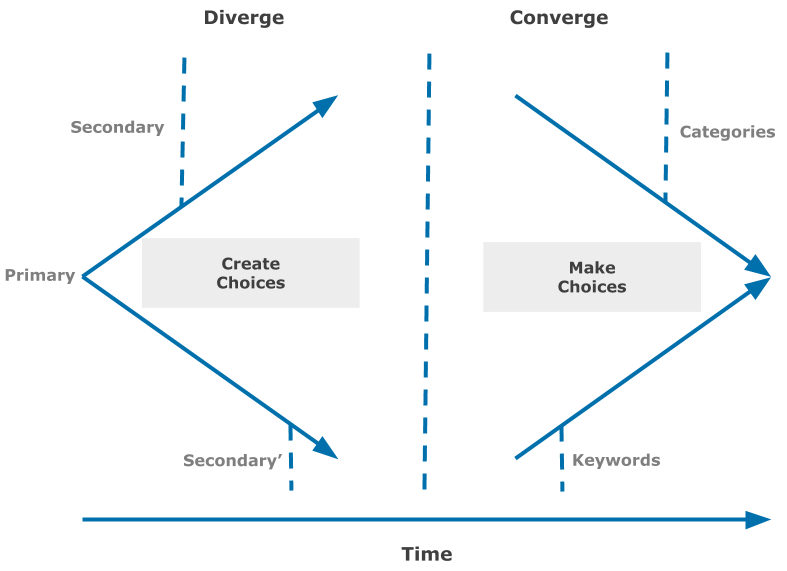
\includegraphics[width=0.75\textwidth]{images/diverge-converge.png}
    \caption[Diverge and Converge process for literature review.]{Diverge and
    Converge process. The divergence phase expands the search space from primary
    sources outward; the convergence phase filters by categories and keywords.
    Source: \textcite{botjes_antifragile_2020}.}\label{fig:diverge-converge}
\end{figure}

Both phases were iterative. New sources discovered during convergence sometimes
triggered additional divergence cycles as citation trails revealed unexpected
connections. The path from Team Topologies
\parencite{skelton_team_topologies_2019} to Cognitive Load Theory
\parencite{sweller_cognitive_1988} to distributed cognition
\parencite{hutchins_cognition_1995} exemplifies this iterative process: each
discovery opened new search directions before convergence narrowed the focus.

\subsubsection{Search Strategies}

Three complementary strategies populated the diverge-converge process.

\textbf{Systematic database search.} An EBSCO host search (June 2025) targeted
top Information Systems journals using combinations of ``enterprise
architecture,'' ``reference architecture,'' ``generative AI,'' and ``large
language models''\footnote{EBSCO host advanced search conducted on June 8, 2025,
    resulted in 0 publications using the query: ((enterprise architecture OR ea
    practice) AND (gen ai OR generative artificial intelligence OR llm OR large
    language models)) AND SO (MIS Quarterly Executive OR Information Systems
    Research OR Journal of the Association for Information Systems OR European
    Journal of Information Systems). Filters applied: peer-reviewed articles,
    publication date from January 1, 2020, to June 8, 2025.}.
The near-zero results confirmed the research gap that motivates this study.

\textbf{Backward and forward citation tracing.} Foundational works served as
primary sources for snowball searches. Starting from
\textcite{zachman_zachman_1987} and \textcite{kotusev_enterprise_2018} for
Enterprise Architecture (EA), \textcite{hutchins_cognition_1995} and
\textcite{hollan_distributed_2000} for distributed cognition,
\textcite{skelton_team_topologies_2019} and
\textcite{sweller_cognitive_1988} for Cognitive Load Theory, and
\textcite{angelov_framework_2012} and \textcite{cloutier_concept_2010} for
Reference Architectures, citation tracing identified additional sources across
these domains. This strategy proved the most productive, yielding the majority
of the theoretical foundation's sources.

\textbf{Practitioner and grey literature.} Industry reports from the
International Energy Agency \parencite{iea_energy_2025}, McKinsey
\parencite{mckinsey_cost_2025}, Microsoft \parencite{microsoft_wti_2025}, and
Stack Overflow developer surveys \parencite{stack_overflow_2024,
stack_overflow_2025} provided empirical context for GenAI adoption trends and
infrastructure investment data not yet covered in peer-reviewed outlets.

Source selection prioritized peer-reviewed publications. Grey literature was
used only for adoption statistics and infrastructure data. The resulting
theoretical foundation (Section~\ref{sec:theoretical-background}) synthesizes
these sources into the five constructs and integrating lens that inform the
conceptual model (Section~\ref{sec:conceptual-model}).

\subsection{Research Implementation}

This subsection describes the expert panel selection, the hybrid round
structure, data collection and analysis procedures, and detailed round
protocols.

\subsubsection{Expert Panel Selection}\label{subsec:expert-panel}

The expert panel was designed for 8--12 EA practitioners selected through
purposive sampling \parencite{patton_qualitative_2015}. Eight participated in
Round~1, ten of twelve invited joined Round~2, and seven of ten invited
attended Round~3. Inclusion required current
hands-on experience using GenAI in EA practice for at least six months and
minimum five years as an EA practitioner to ensure foundational expertise.
Candidates also needed active involvement in Reference Architecture
development and willingness to participate across rounds. Consistent with
\textcite{kotusev_enterprise_2018}'s finding that architectural artifacts involve
distributed authorship, the panel deliberately includes professionals beyond the
``enterprise architect'' title. Participants hold roles including enterprise
architect, solution architect, platform engineer, enterprise data architect,
software architect, and freelance architectural consultant. This role diversity
reflects how RA development unfolds in practice across organizational
boundaries.

For Round~2, the panel was deliberately expanded from the original eight
participants to twelve invitees (five returning from Round~1, seven new).
This expansion served a methodological purpose: pattern validation benefits
from perspectives not anchored to the respondents' own Round~1 submissions,
reducing confirmation bias in category assessment. All new participants met
the same inclusion criteria. Ten of twelve attended. For Round~3, all seven
participants were returning from earlier rounds, ensuring continuity during
the final convergence phase.

The panel composition seeks diversity across four dimensions: industry sectors
(financial services, retail, technology, government), organizational size (SME
to Fortune 500), geographic distribution within European timezone constraints,
and varying levels of GenAI integration depth.
This sample size aligns with \textcite{skulmoski_delphi_2007}, who suggest
that 8--12 experts provide sufficient diversity while enabling meaningful
synchronous interaction. This sampling strategy prioritises information richness
and expert insight over statistical representativeness
\parencite{patton_qualitative_2015}; the resulting panel captures frontier
practice among active GenAI adopters rather than the breadth of the EA
practitioner population.

\subsubsection{Hybrid Delphi Round Structure}

The study combines asynchronous and synchronous elements, moving from
individual discovery to collective sensemaking.
Figure~\ref{fig:delphi-process} shows the complete process flow across all
three rounds.

\begin{figure}[!ht]
    \centering
    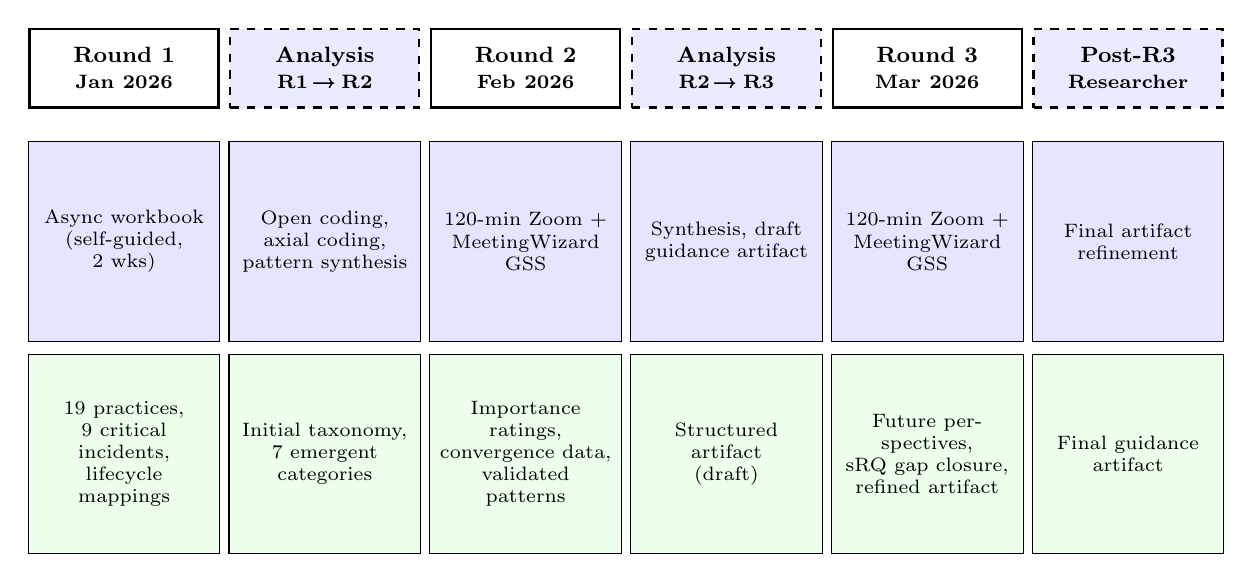
\begin{tikzpicture}[
        % Round nodes: solid border, white fill
        round/.style={rectangle, draw=black, thick, fill=white,
            minimum width=2.4cm, minimum height=1.0cm,
            align=center, font=\footnotesize\bfseries},
        % Analysis nodes: dashed border, light fill
        analysis/.style={rectangle, draw=black, thick, dashed, fill=blue!8,
            minimum width=2.4cm, minimum height=1.0cm,
            align=center, font=\footnotesize\bfseries},
        % Detail and output boxes use a fixed-size \vbox so ALL boxes are
        % exactly the same height regardless of content (5 lines max).
        detail/.style={rectangle, draw=black, fill=blue!10,
            minimum width=2.4cm,
            font=\scriptsize, text width=2.2cm, align=center,
            execute at begin node={\vbox to 2.3cm\bgroup\vfil},
            execute at end node={\vfil\egroup}},
        output/.style={rectangle, draw=black, fill=green!8,
            minimum width=2.4cm,
            font=\scriptsize, text width=2.2cm, align=center,
            execute at begin node={\vbox to 2.3cm\bgroup\vfil},
            execute at end node={\vfil\egroup}},
        ]

        % Column x-coordinates (evenly spaced to fit within \textwidth)
        \def\colsep{2.55cm}
        % Row y-coordinates (spacing for 6-line boxes)
        \def\rowB{-2.2}
        \def\rowC{-4.9}

        % === Top row: phase headers ===
        \node[round] (r1) at (0,0) {Round~1\\{\scriptsize Jan 2026}};
        \node[analysis] (a12) at (\colsep,0) {Analysis\\{\scriptsize R1\,\textrightarrow\,R2}};
        \node[round] (r2) at (2*\colsep,0) {Round~2\\{\scriptsize Feb 2026}};
        \node[analysis] (a23) at (3*\colsep,0) {Analysis\\{\scriptsize R2\,\textrightarrow\,R3}};
        \node[round] (r3) at (4*\colsep,0) {Round~3\\{\scriptsize Mar 2026}};
        \node[analysis] (post) at (5*\colsep,0) {Post-R3\\{\scriptsize Researcher}};

        % === Middle row: method / format ===
        \node[detail] (d1) at (0,\rowB) {Async workbook\\(self-guided, 2 wks)};
        \node[detail] (d12) at (\colsep,\rowB) {Open coding,\\axial coding,\\pattern synthesis};
        \node[detail] (d2) at (2*\colsep,\rowB) {120-min Zoom +\\MeetingWizard GSS};
        \node[detail] (d23) at (3*\colsep,\rowB) {Synthesis, draft\\guidance artifact};
        \node[detail] (d3) at (4*\colsep,\rowB) {120-min Zoom +\\MeetingWizard GSS};
        \node[detail] (dpost) at (5*\colsep,\rowB) {Final artifact\\refinement};

        % === Bottom row: key outputs ===
        \node[output] (o1) at (0,\rowC) {19 practices,\\9 critical incidents,\\lifecycle mappings};
        \node[output] (o12) at (\colsep,\rowC) {Initial taxonomy,\\7 emergent\\categories};
        \node[output] (o2) at (2*\colsep,\rowC) {Importance ratings,\\convergence data,\\validated patterns};
        \node[output] (o23) at (3*\colsep,\rowC) {Structured artifact\\(draft)};
        \node[output] (o3) at (4*\colsep,\rowC) {Future perspectives,\\sRQ gap closure,\\refined artifact};
        \node[output] (opost) at (5*\colsep,\rowC) {Final guidance\\artifact};

    \end{tikzpicture}
    \caption[Delphi process flow with data progression across three rounds.]{Delphi process flow with data progression. Three expert rounds (solid borders) alternate with researcher analysis phases (dashed borders). The middle row (blue) shows the method used in each phase; the bottom row (green) shows the key outputs.}\label{fig:delphi-process}
\end{figure}

\textbf{Round~1 (Asynchronous, January 2026)}: Individual exploration over two weeks

\begin{enumerate}
    \item Participants received a discovery workbook via email
    \item Completed structured sections at their own pace
    \item Documented GenAI practices with rich contextual detail
    \item Provided narrative accounts of critical incidents
    \item Rated confidence and maturity of their practices
\end{enumerate}

\textbf{Rounds~2--3 (Synchronous, February--March 2026)}: Collective refinement

\begin{enumerate}
    \item 120-minute online sessions using Zoom\footnote{Zoom Video Communications: \url{https://zoom.us/}} for video conferencing and MeetingWizard\footnote{MeetingWizard is a cloud-based Group Support System (GSS) platform that structures sessions through agenda creation, anonymous brainstorming, structured voting, and real-time result aggregation, automatically generating reports that capture all discussions and outcomes. See \url{https://www.meetingwizard.nl/en/}} for group deliberation
    \item Real-time validation and exploration of emergent patterns
    \item Dynamic consensus building with technological support
    \item Progressive refinement of guidance artifact
\end{enumerate}

\subsubsection{Data Collection and Analysis}

Each round yields progressively more structured data.

In the asynchronous Round~1, participants describe two to five discovered
practices with step-by-step narratives and genesis stories. They map each
practice to RA lifecycle phases and share three to five critical incidents
(success and failure stories with supporting evidence). They also complete
impact assessments covering time, quality, and role changes; document
challenges and workarounds; and contribute emergent wisdom, including
counterintuitive discoveries and predictions about future practice evolution.

The synchronous Rounds~2--3 generated convergence data through structured GSS
activities. Participants rated the importance of emergent practice categories
on five-point scales and contributed to brainstorms on lifecycle mapping,
practice changes, and trust calibration. Facilitated flipboard discussions
explored boundary conditions and cross-role dynamics. Priority voting
established collective importance weighting, while open-ended brainstorm
responses captured why specific practices work or fail in particular contexts.
Throughout these rounds, participants contributed refinements to the emerging
guidance artifact.

\subsubsection{Round Protocols}

This subsection details the protocol for each round: Round~1 (asynchronous
discovery), Round~2 (synchronous validation), and Round~3 (synchronous final
refinement).

\textbf{Round~1: Asynchronous Exploration (January 2026)}

\textbf{Objective}: Open discovery of emerging practices without researcher framing

\paragraph{Two-Week Structure}

Round~1 gives participants two weeks to complete a discovery workbook at their
own pace. No preliminary artifact or taxonomy is presented; the workbook uses
sensitizing prompts that guide exploration without suggesting predetermined
categories. Guided prompts ensure comparable data across participants, while
free-text responses let practitioners describe practices in their own terms.
Table~\ref{tab:r1-timeline} shows the timeline.

\begin{table}[h]
    \centering
    \caption{Round~1 Timeline and Activities}
    \label{tab:r1-timeline}
    \begin{tabular}{|p{2cm}|p{4cm}|p{4cm}|p{4cm}|}
        \hline
        \textbf{Day}                                                    & \textbf{Activity}       & \textbf{Deliverable}                    & \textbf{Expected Output}           \\
        \hline
        Day 1                                                           & Launch exploration      &
        \begin{itemize}[leftmargin=*,topsep=0pt,itemsep=0pt]
            \item Problem context document
            \item Discovery workbook
            \item Standard RA lifecycle
        \end{itemize} & Participant orientation                                                                                                           \\
        \hline
        Days 2--10                                                       & Self-guided discovery   & Participants complete workbook sections & 2--5 core practices per participant \\
        \hline
        Day 11--12                                                       & Reflection prompts      & Additional prompts for unexplored areas & Completeness check                 \\
        \hline
        Day 13--14                                                       & Submission deadline     & Completed workbooks                     & \textasciitilde19 total practices  \\
        \hline
        Days 15--25                                                      & Intensive analysis      & Pattern emergence and synthesis         & Initial taxonomy and guidance \\
        \hline
    \end{tabular}
\end{table}

\paragraph{Discovery Workbook Design}

The discovery workbook serves as the primary data collection instrument,
structured to guide systematic exploration while avoiding constraining
participants' responses. The workbook employs a progressive structure that
moves from context setting through practice discovery to reflective
sensemaking.

We deliberately framed the workbook scope as ``Software Architecture / Solution
Design work'' rather than ``Enterprise Architecture.'' This choice reflects a
terminological broadening, not a scope expansion. Practitioners who create,
update, and govern Reference Architectures often describe this work as
``solution design'' or ``software architecture'' rather than ``RA development.''
A strict EA framing risked excluding professionals who materially shape
architectural artifacts but do not identify as enterprise architects: solution
architects, platform engineers, and senior developers whose daily work involves
Reference Architectures
\parencite[see Section~\ref{sec:theoretical-background}]{kotusev_enterprise_2018}.

This terminological broadening introduces a validity tension. Practices
discovered under a ``Software Architecture'' framing may extend beyond
RA-specific work into general architectural practice, blurring the boundary
with the research question's ``EA practitioners'' scope. Two instrument design
features mitigate this risk. First, Part~C of the workbook requires
participants to map each practice to eight RA lifecycle phases, structurally
anchoring reported practices to RA development regardless of the terminology
used to invite participation. Second, the R2 validation session evaluated
practices specifically in the context of RA development: ten participants from
diverse architectural roles all recognized their practice in the workbook
prompts. By meeting practitioners in their own terminology while anchoring
responses to the RA lifecycle, the instrument captured practices that a narrower
EA-only framing might have excluded without sacrificing scope specificity.

The workbook comprises seven parts. Part~A establishes the
participant's GenAI tooling, experience level, and organizational context.
Part~B (Practice Archaeology) forms the core discovery section, prompting
participants to recall genesis moments and systematically document each named
practice with its problem, step-by-step process, effectiveness rate, and
failure modes. Part~C asks participants to map their practices to eight RA
lifecycle phases and identify tasks that must remain human-performed. Part~D
solicits three to five critical incident narratives with structured fields for
context, action, result, insight, and supporting evidence. Part~E captures
impact reflections across three dimensions: time and effort, quality and
completeness, and role evolution. Part~F documents challenges encountered along
with workarounds and capability wishes. Part~G elicits emergent wisdom,
including advice for colleagues, counterintuitive discoveries, and twelve-month
predictions. This structure balances guided prompts for cross-participant
comparability with free-text responses that allow practitioners to describe
practices in their own terms. The complete workbook instrument is provided in
\ref{app:workbook}.

\paragraph{Data Collection Platform}

The workbook was deployed as a structured Word document distributed via email,
providing:
\begin{itemize}
    \item Completion over multiple sessions at the participant's own pace
    \item Structured sections guiding progressive exploration
    \item Rich text formatting for detailed descriptions
    \item Clear section delineation to encourage completeness
\end{itemize}

\paragraph{Outputs}

Round~1 yielded:
\begin{itemize}
    \item 19 distinct practice descriptions (\textasciitilde2--3 per participant $\times$ 8 participants)
    \item 9 critical incident narratives with evidence
    \item Practice-to-lifecycle mappings across all workbook sections
    \item 12 challenges with workarounds
    \item 8 sets of emergent wisdom and predictions
\end{itemize}

This dataset underwent intensive analysis (Days 15--25) to identify emergent
patterns, create an initial practice taxonomy, and develop the first version of
the guidance artifact for validation in Round~2.

\textbf{Round~2: Synchronous Pattern Validation (4 February 2026)}

\textbf{Objective}: Validate emergent patterns from Round~1 and explore variations

Round~2 was conducted as a 120-minute synchronous session via Zoom\footnote{\url{https://zoom.us/}} with
MeetingWizard\footnote{\url{https://www.meetingwizard.nl/en/}} GSS technology \parencite[see also][for a recent application in EA research]{nieuwenhuis_towards_2025}. Ten of twelve invited participants joined. The
session presented emergent practice categories synthesized from Round~1
analysis for collective validation. The planned 15-step protocol was partially
executed during the synchronous session: Steps~1--7 (opening, practice
presentation, brainstorm on reactions and gaps, flipboard discussion on
practice categories, importance voting, lifecycle mapping brainstorm, and
before/after brainstorm) were completed in real time. Two remaining voting
steps (Change Significance and Heuristic Agreement) were collected
asynchronously afterward; all ten participants completed these votes. The
session generated convergence data on practitioner agreement levels and
cross-cutting patterns, providing input for the evolving guidance artifact.

\textbf{Round~3: Synchronous Final Refinement (4 March 2026)}

\textbf{Objective}: Gather future-oriented data, address remaining sub-research-question gaps, and collect input for the final guidance artifact

Round~3 was the final synchronous session, building on the validated practice
categories from Round~2. Seven of ten invited participants attended the
120-minute session; all seven were returning participants from earlier rounds.
The session was designed around three objectives. First, it aimed to elicit
forward-looking perspectives on how GenAI practices in RA development may
evolve. Second, it collected data for sub-research-questions not yet fully
addressed, particularly sRQ3 on sensemaking and sRQ4 on systematization.
Third, it gathered practitioner input to refine the draft guidance artifact.
Procedural deviations from the planned 16-step protocol are documented in
Section~\ref{subsec:data-limitations}.

Preliminary analysis of Rounds~1 and~2 had surfaced cross-role dynamics as an
emergent theme. \textcite{kotusev_enterprise_2018}'s finding that architectural
artifacts involve distributed authorship provided theoretical grounding for
this observation. This motivated three targeted R3 probes: how developer-level
GenAI use informs architectural artifacts bottom-up, what traceability
mechanisms practitioners employ when GenAI distributes authorship across roles,
and where governance friction arises when non-architects produce architectural
outputs.

\subsection{Data Analysis Framework}

The hybrid design requires distinct analytical approaches for the discovery
phase versus the convergence phases:

\subsubsection{Round~1 Discovery Analysis (Days 15--25)}

The discovery analysis proceeds through four phases over Days 15--25.
Phase~1 (data immersion) involves reading all workbooks, memoing first
impressions, and creating participant profiles. Phase~2 (open coding) fractures
data into discrete concepts using line-by-line, in-vivo, incident, process,
and emotion coding \parencite{charmaz_constructing_2014}. Phase~3 (pattern
emergence) applies axial coding: identifying relationships between practices,
comparing across participants, and clustering similar practices into
preliminary categories.

These coding phases produced four coding dimensions that
structure the Round~1 findings reported in Section~\ref{sec:results}:
\emph{interaction patterns} (how practitioners engage GenAI, from research
assistant to deep integration), \emph{distribution of cognitive tasks} (which
tasks practitioners delegate versus retain), \emph{engagement quality} (the
degree of active oversight practitioners maintain over GenAI outputs), and
\emph{practice reconfiguration} (how established workflows changed with GenAI
adoption). These dimensions emerged abductively: initial codes were derived
inductively from practitioner language, then organized through constant
comparison against the distributed cognition lens established in
Section~\ref{sec:conceptual-model}
\parencite{charmaz_constructing_2014, patton_qualitative_2015}. Together, the
four dimensions provided a consistent analytical vocabulary for coding all 19
discovered practices and the cross-cutting patterns across the panel.

Phase~4 (synthesis) creates a practice taxonomy, maps practices to RA
lifecycle phases, documents variation patterns, and prepares validation
materials for Round~2. Three analytical decisions guide the process:
practitioner language is preserved in category names, minority practices are
kept even when mentioned by few participants, and contradictions are documented
as variation points rather than treated as errors.

In addition to these coding categories, cross-role dynamics serve as an
emergent analytical dimension. Round~1 revealed that practitioners routinely
described practices crossing traditional role boundaries; what the coded
analysis labels Pattern~4. Round~2's panel diversity reinforced this
observation: inside-out workflows and collective decision capture surfaced
precisely because participants held varied architectural roles. This dimension
complements the existing coding categories (in-vivo, incident, process,
emotion) as a thematic lens for identifying how GenAI redistributes
architectural work across organizational roles.
\textcite{hollan_distributed_2000}'s distributed cognition framework (where
cognitive processes distribute across individuals, artifacts, and
environments) grounds this analytical choice theoretically.

\subsubsection{Between-Round Analysis (Synchronous Rounds)}

\paragraph{Round~2 $\rightarrow$ 3 Analysis}
\begin{itemize}
    \item Synthesized Round~2 importance ratings and variability profiles per
          practice category
    \item Confirmed seven practice categories; no category revisions required
    \item Prepared structured artifact with six elements per practice
          (description, lifecycle phases, guidance level, experience indicators,
          verification patterns, cross-role considerations)
    \item Designed targeted Round~3 probes based on emergent gaps (cross-role
          dynamics, trust calibration)
\end{itemize}

\paragraph{Round~3 Final Analysis}
\begin{itemize}
    \item Calculated consensus and variability metrics for all Round~3 voting
          items (heuristics, cross-role patterns, guidance priorities)
    \item Organized verification heuristics into tiers based on consensus strength
    \item Analyzed cross-role pattern significance; noted high variability as
          context-dependent rather than universal
    \item Integrated guidance element priority ratings into final artifact
          structure
    \item Finalized guidance artifact incorporating all three rounds of data
\end{itemize}

\subsection{Quality Criteria}

This subsection addresses methodological rigor, trustworthiness, and the
study's limitations and delimitations.

\subsubsection{Rigor in Exploratory-Convergent Delphi}

Discovery validity in Round~1 is established through open-ended exploration
where no researcher-imposed categories constrain what participants can report.
Rich description through detailed narratives enables thick interpretation of
practitioner experiences. Evidence grounding ensures that actual prompts and
outputs support practitioner claims. Negative case analysis explicitly solicits
failures and challenges alongside successes.

Convergence validity in Rounds~2--3 relies on four mechanisms. Member checking
ensures participants validate interpretations at each round. Consensus metrics
provide transparent reporting of agreement levels. Variation documentation
preserves divergence without forcing artificial agreement, and progressive
refinement enables iterative improvement across multiple rounds.

\subsubsection{Trustworthiness Criteria}

Delphi studies face established methodological critiques, particularly
concerning researcher influence during synthesis, pressure toward artificial
consensus, and arbitrary definitions of expertise
\parencite{linstone_delphi_1975, okoli_delphi_2004}. Following
\textcite{lincoln_naturalistic_1985}, this research addresses these risks
through four trustworthiness criteria.

\textbf{Credibility} addresses the risk of researcher bias in interpreting and
synthesizing participant responses. This study establishes credibility through
prolonged engagement across three rounds over four months, allowing the researcher
to develop deep familiarity with practitioner perspectives. Triangulation across
multiple data types (narratives, ratings, and group discussions) reduces
dependence on any single source. Member checking at each round ensures
participants validate researcher interpretations before subsequent rounds build
upon them. The analysis explicitly seeks negative cases, including failures and
divergent views, rather than selecting only confirmatory evidence. Regular peer
debriefing with the research supervisor provides external challenge to emerging
interpretations.

\textbf{Transferability} addresses the risk that arbitrary or unclear expert
selection limits the applicability of findings to broader contexts. The research
provides thick description of participant organizational contexts, enabling
readers to assess relevance to their own situations. Boundary conditions for
guidance applicability are specified explicitly, acknowledging where practices transfer and where they do not. Documentation of practice variations across contexts
preserves important distinctions rather than forcing premature generalization.
The clear articulation of participant selection criteria in
Section~\ref{sec:methodology} allows readers to evaluate the expertise base
underlying the findings.

\textbf{Dependability} addresses the risk of subjective analytical decisions
lacking transparency. A comprehensive audit trail documents all analytical
decisions, from initial coding through pattern synthesis to final guidance
formulation. Code-recode reliability checks at two-week intervals ensure
consistency in the researcher's interpretive framework over time. External
advisor review of the coding framework provides independent validation of
analytical categories. Version control for the guidance artifact (tracking its
evolution across rounds) makes visible how collective input shaped the
final output.

\textbf{Confirmability} addresses the risk that controlled feedback creates
pressure toward artificial consensus, suppressing minority views. Reflexive notes captured at key analytical decision points document the
researcher's evolving assumptions and their potential influence on
interpretation. Direct
participant quotes support all substantive interpretations, grounding claims in
participant voice rather than researcher inference. Divergent views are
explicitly preserved in the final guidance rather than eliminated in pursuit of
false unanimity. Raw data remains available for audit, enabling independent
verification of the analytical process.

\subsubsection{Limitations}

The methodology faces both methodological and scope limitations.
Methodologically, discovery is limited to current practitioners, missing the
perspective of non-adopters who tried and rejected GenAI integration.
Practices are self-reported without direct observation, introducing recall
bias. Social desirability bias likely persists despite anonymity measures.
The synthesis between rounds requires researcher interpretation, creating
opportunities for unintentional influence.

In terms of scope, the focus on the RA lifecycle excludes other EA activities
where GenAI integration manifests differently. European timezone constraints
limit global representation of the expert panel. The research captures current
practices rather than future possibilities, providing a snapshot of an evolving
phenomenon. Individual practices receive emphasis over organizational adoption
patterns.

\subsubsection{Delimitations}

This research establishes purposeful boundaries to maintain focus and
feasibility. The technology scope limits GenAI to LLM-based systems, excluding
other AI types such as computer vision or predictive analytics. The artifact
focus uses Reference Architecture as the primary lens rather than examining all
EA deliverables.

The practice emphasis prioritizes discovery of what practitioners are currently
doing over prescription of what they should do. The outcome orientation favors
practical guidance for the EA community over purely theoretical contribution.

\subsection{Ethical Considerations}

The research adheres to university ethical guidelines and professional
standards:

\begin{enumerate}
    \item \textbf{Informed Consent}: Participants receive comprehensive information about the exploratory nature, time commitment, and data usage. Consent explicitly covers the iterative nature of the Delphi process.

    \item \textbf{Anonymity Protection}: Individual practices are not attributed to specific participants. The Group Support System ensures anonymous contribution during synchronous sessions. Only aggregated findings appear in publications. Where individual participant quotations are presented, participants are identified by codes (P1--P4) to preserve anonymity.

    \item \textbf{Intellectual Property}: Clear agreement that shared practices become collective knowledge for the EA community. Organizations retain rights to their specific implementations while contributing patterns to the common body of knowledge.

    \item \textbf{Right to Withdraw}: Participants can exit the study at any point without consequence. Partial participation is valued and included where appropriate.

    \item \textbf{Reciprocity}: All participants receive the final guidance document and summary findings. Acknowledgment offered (with permission) in publications.
\end{enumerate}

Full disclosure of Generative AI tool usage throughout this research is provided
in \ref{app:genai}.

\subsection{Research Quality Criteria}

Beyond the qualitative rigor criteria addressed above (credibility,
transferability, dependability, confirmability), two additional frameworks
inform the quality standards of this research.

\textcite{recker_scientific_2021} identifies four principles for scientific
research: replicability, independence, precision, and falsifiability. This
study addresses each as follows. \textbf{Replicability}: the methodology
chapter documents protocols, instruments (Appendix~\ref{app:workbook}), and
analytical procedures in sufficient detail for independent replication.
\textbf{Independence}: the Delphi design uses anonymous input and controlled
feedback to minimize researcher influence on participant responses.
\textbf{Precision}: coding schemes, rating scales, and consensus thresholds
are defined explicitly. \textbf{Falsifiability}: the study's claims are
bounded by the data; negative cases and divergent views are preserved rather
than suppressed, and limitations are stated explicitly.

The FAIR principles \parencite{wilkinson_fair_2016} (Findable, Accessible, Interoperable, Reusable) guide the
research data management strategy. Research instruments and the
machine-readable guidance artifact are designed for reuse. The YAML artifact
in particular enables computational processing by other researchers. Upon
completion and grading, the research repository, including the machine-readable
artifact,\footnote{\url{https://github.com/thiagoavadore/thesis_2024-2026_antwerp_thesis_GenAIPracticeVacuum/blob/main/guidance-artifact.yaml}}
will be made publicly accessible to support transparency and reproducibility.

\subsection{Timeline and Logistics}

Table~\ref{tab:timeline} presents the research timeline spanning September 2025
through May 2026.

\begin{table}[htbp]
    \centering
    \caption{Research Timeline}\label{tab:timeline}
    \begin{tabular}{|l|l|l|}
        \hline
        \textbf{Phase} & \textbf{Activities}                           & \textbf{Timeline} \\
        \hline
        Preparation    & Recruitment, platform setup, workbook testing & September 2025    \\
        \hline
        Round~1        & Async discovery weeks + intensive analysis    & January 2026      \\
        \hline
        Round~2        & Pattern validation session + analysis         & February 2026     \\
        \hline
        Round~3        & Final round + synthesis                       & March 2026        \\
        \hline
        Dissemination  & Guidance publication and community sharing    & April--May 2026   \\
        \hline
    \end{tabular}
\end{table}

